Consider a unity gain feedback system:\begin{minipage}{2in}
\resizebox{2in}{!}{
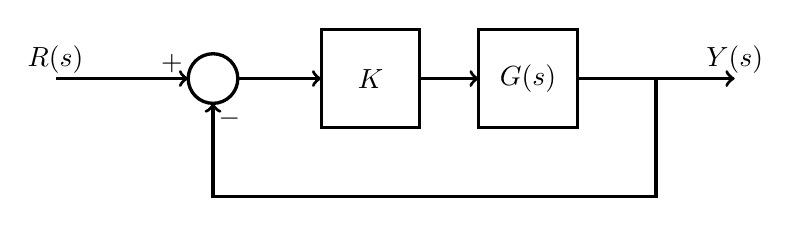
\begin{tikzpicture}[scale=1,inner sep=0pt,outer sep=0pt,very thick,
sysblock/.style={draw,rectangle,inner sep=2pt,minimum width=1.25cm,minimum height=1.25cm,inner sep=4pt, very thick}]
\draw (2,0) node[draw,circle] (sum1) {$\rule{0pt}{18pt}$};
\draw (4,0) node[sysblock] (K) {$K$};
\draw (6,0) node[sysblock] (G) {$G(s)$};
\draw[->] (0,0) node[above=2pt] {$R(s)$} -- (sum1.180) node[above left=2pt] {$+$};
\draw[->] (sum1.0)  -- (K.180);
\draw[->] (K.0) -- (G.180);
\draw[->] (G.0) -- ++(2,0) node[above=2pt] {$Y(s)$};
\draw[->] (G.0) ++(1,0) -- ++(0,-1.5) -| (sum1.-90) node[below right=2pt] {$-$};
\end{tikzpicture}}
\end{minipage}
The Bode plot of $G(s)$, which has one pole at $s=0$ and no poles in the open right half plane, is shown below. {\em Note that this is the Bode plot of the loop gain when $K=1$.} You wish to design a proportional control system such that $\tr=0.44$s. 

\includegraphics[width=5.5in]{\mainfolder/LectureNotes/\lecturefolder/HomeworkProblems/Problem03/bode3.pdf}

\begin{enumerate}[(a)]
\item What gain should you choose to achieve this design specification?
\item What is the resulting phase and gain margin for this design?
\end{enumerate}

